% Compile with: xelatex egg-fried-rice.tex
\documentclass[11pt]{article}

\usepackage[margin=1in]{geometry}
\usepackage{amsmath,amssymb}
\usepackage{pgfplots}
\pgfplotsset{compat=1.18}
\usepackage{hyperref}
\usepackage{authblk}
\usepackage{cite}
\usepackage{fontspec}
\usepackage{xeCJK}
\setCJKmainfont{PingFang SC}[BoldFont={PingFang SC},ItalicFont={PingFang SC}]

\hypersetup{colorlinks=true, linkcolor=blue, citecolor=blue, urlcolor=blue}

\title{An Optimal Stirring Intensity for Complete Egg--Rice Bonding\\ in Fried Rice: A Percolation--Coagulation Model}

\author[1]{Koutian Wu}
\affil[1]{Independent Research (GitHub: \href{https://github.com/ktwu01}{ktwu01})}

\date{}

\begin{document}
\maketitle

\begin{abstract}
Properly made egg fried rice (蛋炒饭) requires every grain of rice to be bonded to egg, with neither bare rice grains nor isolated clumps of egg. This is, on its face, a materials-science problem: a protein film undergoing a coagulation phase transition must wet and adhere to a granular solid under mechanical agitation. We propose a four-part model that treats egg coagulation as an Avrami-type nucleation-and-growth process rather than simple first-order kinetics, models rice-grain surface coverage as the outcome of two competing stirring-driven processes (collision-driven contact versus shear-driven fragmentation), imposes a stoichiometric ceiling set by the egg-to-rice mass ratio, and defines macroscopic "bonding" via a percolation-style criterion on the mean and variance of coverage across grains, rather than the mean alone. The central quantitative prediction is that stirring intensity has a genuine interior optimum $I^*$, rather than a monotonic effect in either direction, and that $I^*$ shifts predictably with cook time. We provide closed-form and numerically integrated results, an open-source interactive simulator, and a discussion of what would be required to move this model from plausible to experimentally validated.
\end{abstract}

\section{Introduction}

Home cooks and professional chefs agree on several heuristics for egg fried rice: use day-old refrigerated rice, keep the wok hot, and stir promptly and vigorously. What is missing from this folklore is any predictive account of \emph{why} these heuristics work, or what would happen if they were pushed to their extremes. In particular, the endpoint condition of a perfectly made batch is rarely stated precisely. We take it to be this: every rice grain is coated by coagulated egg, and no egg exists as an isolated mass separate from rice. We refer to this as the \emph{fully bonded} state.

This problem was first posed informally in a conversation with a large language model in October 2023 \cite{gfr2023}, which produced a first-pass model treating egg coagulation as a simple phase transition and stirring as a monotonically \emph{negative} influence on egg--rice contact probability. That model is a reasonable starting sketch, but has three specific weaknesses that motivate the present work:

\begin{enumerate}
    \item Its coagulation kinetics assumed a bare first-order relaxation, $d\phi/dt = r(T)(1-\phi)$, which implies the fastest coagulation rate occurs at $t=0$. Protein coagulation is a nucleation-and-growth process and is better described by Avrami-type kinetics, which predict an induction period followed by acceleration \cite{avrami1939}.
    \item Its stirring term, $P = P_0 e^{-I/I_0}$, asserts that \emph{more} stirring always yields \emph{less} egg--rice contact, with no stated mechanism. This directly conflicts with the common failure mode of under-stirred fried rice, where large unmixed patches of egg and rice never touch at all.
    \item It provided no criterion for deciding when the fully bonded state has actually been reached. Multiplying a contact probability by a coagulation rate produces a number, but that number was never connected back to the stated goal of ``no isolated rice grains, no isolated egg.''
\end{enumerate}

We address each of these in turn.

\section{Model}

\subsection{Coagulation as nucleation and growth}

We treat egg coagulation as a phase transformation and describe the coagulated volume fraction $\phi(t)$ using Avrami kinetics,
\begin{equation}
    \phi(t) = 1 - \exp\!\left[-\big(k(T)\,t\big)^n\right], \qquad k(T) = A\, e^{-E_a / R T},
    \label{eq:avrami}
\end{equation}
where $k(T)$ follows an Arrhenius temperature dependence with activation energy $E_a$, and $n$ is the Avrami exponent governing the geometry of nucleation and growth. Unlike the first-order model $\phi_{\text{1st}}(t) = 1 - e^{-k t}$, which has its steepest slope at $t = 0$, Eq.~\eqref{eq:avrami} produces a sigmoidal curve with an induction period, consistent with the observation that egg white does not visibly set the instant it contacts a hot wok. Figure~\ref{fig:avrami} compares the two forms at a representative wok temperature.

\begin{figure}[htbp]
\centering
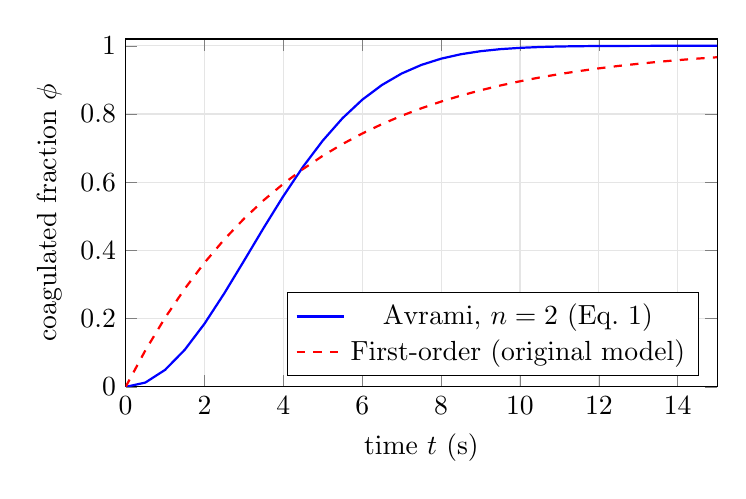
\begin{tikzpicture}
\begin{axis}[
    width=0.75\textwidth, height=6cm,
    xlabel={time $t$ (s)}, ylabel={coagulated fraction $\phi$},
    legend pos=south east, ymin=0, ymax=1.02, xmin=0, xmax=15,
    grid=major, grid style={gray!20}
]
\addplot[thick, blue] coordinates {
(0.0,0.0) (0.5,0.0127) (1.0,0.0499) (1.5,0.1089) (2.0,0.1853) (2.5,0.274) (3.0,0.3694) (3.5,0.4662) (4.0,0.5595) (4.5,0.6457) (5.0,0.7222) (5.5,0.7878) (6.0,0.8419) (6.5,0.8852) (7.0,0.9188) (7.5,0.944) (8.0,0.9623) (8.5,0.9753) (9.0,0.9842) (9.5,0.9902) (10.0,0.994) (10.5,0.9965) (11.0,0.998) (11.5,0.9989) (12.0,0.9994) (12.5,0.9997) (13.0,0.9998) (13.5,0.9999) (14.0,1.0) (14.5,1.0) (15.0,1.0)
};
\addlegendentry{Avrami, $n=2$ (Eq.~1)}
\addplot[thick, red, dashed] coordinates {
(0.0,0.0) (0.5,0.107) (1.0,0.2026) (1.5,0.2879) (2.0,0.3641) (2.5,0.4322) (3.0,0.4929) (3.5,0.5472) (4.0,0.5956) (4.5,0.6389) (5.0,0.6776) (5.5,0.7121) (6.0,0.7429) (6.5,0.7704) (7.0,0.795) (7.5,0.8169) (8.0,0.8365) (8.5,0.854) (9.0,0.8696) (9.5,0.8836) (10.0,0.896) (10.5,0.9072) (11.0,0.9171) (11.5,0.926) (12.0,0.9339) (12.5,0.941) (13.0,0.9473) (13.5,0.9529) (14.0,0.958) (14.5,0.9625) (15.0,0.9665)
};
\addlegendentry{First-order (original model)}
\end{axis}
\end{tikzpicture}
\caption{Coagulated egg fraction $\phi(t)$ at $T = 180^\circ$C under Avrami nucleation-and-growth kinetics versus the naive first-order model. The Avrami curve exhibits an induction period absent from the first-order form.}
\label{fig:avrami}
\end{figure}

\subsection{Competing effects of stirring}

Let $\theta_i \in [0,1]$ denote the fraction of grain $i$'s surface covered by coagulated egg. We propose that stirring drives two physically distinct, opposing processes: it increases the collision frequency between rice grains and still-fluid egg (building coverage), and it increases the shear stress that tears already-adhered egg film back off a grain's surface (destroying coverage). Taking the collision rate to scale linearly in stirring intensity $I$ and the fragmentation rate to scale quadratically (as shear rate generally does in the dissipation of a viscous film),
\begin{equation}
    \frac{d\theta}{dt} = \beta_0 I \,\big(\theta_{\max} - \theta\big)\,\phi(t) \;-\; \gamma_0 I^2\, \theta,
    \label{eq:coverage}
\end{equation}
where $\beta_0$ and $\gamma_0$ are empirical rate constants and $\theta_{\max}$ is the maximum achievable coverage (Section~\ref{sec:stoich}). Because the fragmentation term grows faster in $I$ than the collision term, Eq.~\eqref{eq:coverage} has no monotonic relationship between $I$ and final coverage at fixed cook time $t_{\text{cook}}$: insufficient stirring never distributes egg over the full rice surface within the available time, while excessive stirring reaches a lower steady-state coverage because it destroys film as fast as it forms it. This produces a genuine interior optimum $I^*(t_{\text{cook}}, T)$, illustrated in Figure~\ref{fig:optimum}.

\begin{figure}[htbp]
\centering
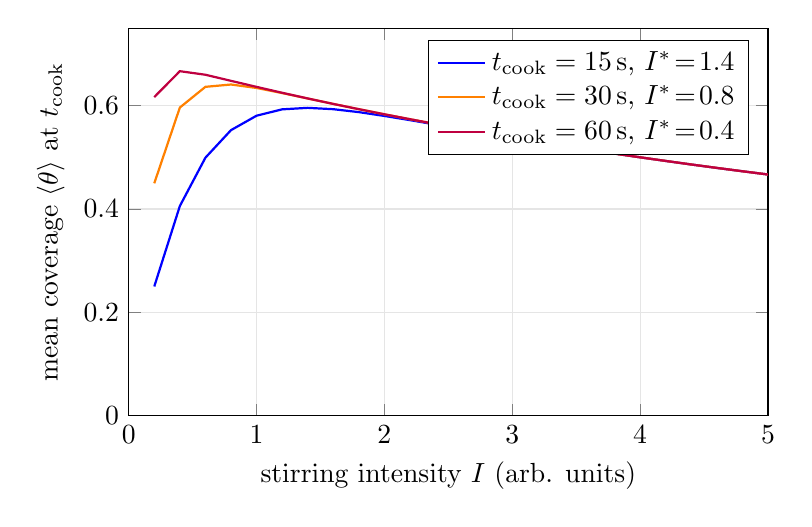
\begin{tikzpicture}
\begin{axis}[
    width=0.8\textwidth, height=6.5cm,
    xlabel={stirring intensity $I$ (arb. units)}, ylabel={mean coverage $\langle\theta\rangle$ at $t_{\text{cook}}$},
    legend pos=north east, ymin=0, ymax=0.75, xmin=0, xmax=5,
    grid=major, grid style={gray!20}
]
\addplot[thick, blue, mark=none] coordinates {
(0.2,0.2499) (0.4,0.4057) (0.6,0.4993) (0.8,0.5526) (1.0,0.5806) (1.2,0.5929) (1.4,0.5958) (1.6,0.5932) (1.8,0.5875) (2.0,0.5801) (2.2,0.572) (2.4,0.5635) (2.6,0.555) (2.8,0.5465) (3.0,0.5383) (3.2,0.5302) (3.4,0.5223) (3.6,0.5147) (3.8,0.5072) (4.0,0.5) (4.2,0.4929) (4.4,0.4861) (4.6,0.4794) (4.8,0.473) (5.0,0.4667)
};
\addlegendentry{$t_{\text{cook}}=15$\,s, $I^*\!=\!1.4$}
\addplot[thick, orange, mark=none] coordinates {
(0.2,0.4497) (0.4,0.5964) (0.6,0.6365) (0.8,0.641) (1.0,0.6343) (1.2,0.6244) (1.4,0.6139) (1.6,0.6034) (1.8,0.5932) (2.0,0.5833) (2.2,0.5738) (2.4,0.5645) (2.6,0.5556) (2.8,0.5469) (3.0,0.5385) (3.2,0.5303) (3.4,0.5224) (3.6,0.5147) (3.8,0.5072) (4.0,0.5) (4.2,0.493) (4.4,0.4861) (4.6,0.4795) (4.8,0.473) (5.0,0.4667)
};
\addlegendentry{$t_{\text{cook}}=30$\,s, $I^*\!=\!0.8$}
\addplot[thick, purple, mark=none] coordinates {
(0.2,0.6167) (0.4,0.6668) (0.6,0.6599) (0.8,0.6481) (1.0,0.6364) (1.2,0.625) (1.4,0.614) (1.6,0.6034) (1.8,0.5932) (2.0,0.5833) (2.2,0.5738) (2.4,0.5645) (2.6,0.5556) (2.8,0.5469) (3.0,0.5385) (3.2,0.5303) (3.4,0.5224) (3.6,0.5147) (3.8,0.5072) (4.0,0.5) (4.2,0.493) (4.4,0.4861) (4.6,0.4795) (4.8,0.473) (5.0,0.4667)
};
\addlegendentry{$t_{\text{cook}}=60$\,s, $I^*\!=\!0.4$}
\end{axis}
\end{tikzpicture}
\caption{Mean coverage $\langle\theta\rangle$ at the end of cooking, as a function of stirring intensity $I$, for three cook times ($T=180^\circ$C, egg:rice mass ratio $r=0.7$). Each curve has an interior maximum: too little stirring is kinetically limited, too much destroys coverage through shear fragmentation. The optimal intensity $I^*$ decreases as available cook time increases, since a longer cook time gives gentler stirring time to reach the same coverage without incurring fragmentation losses.}
\label{fig:optimum}
\end{figure}

\subsection{Stoichiometric ceiling}
\label{sec:stoich}

No amount of favorable kinetics can coat rice grains with egg that is not present. We impose a hard ceiling on achievable coverage set by the egg-to-rice mass ratio $r$,
\begin{equation}
    \theta_{\max}(r) = \min\!\left(1, \frac{r}{r_c}\right),
    \label{eq:stoich}
\end{equation}
where $r_c$ is the mass ratio required to give every grain a complete monolayer. This term is absent from the original model entirely; without it, sufficiently aggressive kinetics parameters would predict complete bonding regardless of how little egg is used, which is physically absurd.

\subsection{A percolation criterion for ``bonded''}

The original question was never actually ``what is the mean coverage,'' but ``are there isolated rice grains or isolated egg.'' This is a statement about the distribution of $\theta$ across the population of grains, not only its mean. We therefore define the fully bonded state as
\begin{equation}
    \text{bonded} \iff \langle \theta \rangle \ge \theta_c \ \ \text{and} \ \ \mathrm{Var}(\theta) \le \mathrm{Var}_c,
    \label{eq:percolation}
\end{equation}
for threshold constants $\theta_c$ and $\mathrm{Var}_c$. A batch with high mean coverage but high variance is not fully bonded in the intended sense: it simply means some grains are completely coated while others remain bare, which is exactly the failure mode the original question sought to exclude. This is, in spirit, a percolation condition: a continuous, sample-spanning egg network requires not just enough egg on average, but enough egg \emph{everywhere}.

\section{Numerical demonstration}

We implemented Eqs.~\eqref{eq:avrami}--\eqref{eq:percolation} as a stochastic per-grain simulation (each grain evolves under Eq.~\eqref{eq:coverage} independently, with a small multiplicative noise term representing local heterogeneity in mixing) and as a deterministic mean-field integration for computing $I^*$. Both are available as an interactive, browser-based simulator with adjustable temperature, stirring intensity, egg:rice ratio, and cook time, at \url{https://github.com/ktwu01/egg-fried-rice-materials-model}. The simulator numerically sweeps $I$ at the current parameter settings and displays $I^*$ live, alongside an animated population of grains colored by instantaneous coverage.

During development of the simulator, an implementation error was identified and corrected: the initial choice of $r_c$ in Eq.~\eqref{eq:stoich} caused $\theta_{\max}$ to saturate at 1 for most of the intended egg:rice ratio range, making the ratio parameter's effect invisible over roughly two-thirds of its range. This was caught by inspection of the rendered simulation rather than by the underlying mathematics, and is a useful reminder that a correct model can still be misrepresented by a poorly calibrated parameter.

\section{Discussion}

The model makes three falsifiable predictions that distinguish it from the original first-order/monotonic-stirring account:
\begin{enumerate}
    \item There exists an interior optimal stirring intensity $I^*$ for any fixed cook time, rather than a monotonic relationship between stirring and bonding quality.
    \item $I^*$ decreases as available cook time increases: a cook working quickly under high heat should stir more vigorously than one working slowly.
    \item Two batches with identical mean egg coverage can differ in whether they are ``fully bonded,'' depending on the variance of coverage across grains — i.e., bonding quality is not fully captured by any single scalar summary such as total egg used.
\end{enumerate}
Testing these predictions experimentally would require frying controlled batches at fixed temperature and egg:rice ratio while varying stirring intensity and cook time, then quantifying coverage by image analysis of photographed samples (e.g., the fraction of each rice grain's visible surface area classified as egg-coated by color thresholding). We have not yet performed such an experiment; the present work should be read as a theoretical framework and simulation, not an experimentally validated result. We regard closing that gap as the natural next step, and the one most likely to determine whether this line of inquiry has any claim to recognition beyond its authors' own amusement.

\section*{Acknowledgments}

This project originated from a conversation with ChatGPT in October 2023, archived in full at \url{https://github.com/ktwu01/egg-fried-rice-materials-model/tree/main/original-2023}. All code, the interactive simulator, and this manuscript's source are released openly at the same repository.

\begin{thebibliography}{9}

\bibitem{gfr2023}
Original conversation, \emph{A Materials-Science Model of Egg Fried Rice}, ChatGPT, October 5, 2023. \url{https://chat.openai.com/share/33bbea16-9508-4c8c-b300-198880b8d434}

\bibitem{avrami1939}
M. Avrami, ``Kinetics of Phase Change. I: General Theory,'' \emph{J. Chem. Phys.} \textbf{7}, 1103 (1939).

\bibitem{stauffer2018}
D. Stauffer and A. Aharony, \emph{Introduction to Percolation Theory}, 2nd ed., Taylor \& Francis (2018).

\end{thebibliography}

\end{document}
